% Tipo de documento (presentación)
\documentclass[10pt, xcolor=table]{beamer}

% Cargar el tema
\usetheme{metropolis}

%  __________
% |          |
% | Paquetes |
% |__________|

% Paquetes de idioma
\usepackage[utf8]{inputenc}
\usepackage[spanish, es-tabla, es-lcroman, es-noquoting]{babel}

% Paquete para código fuente
% LISTINGS
\usepackage{listings}
\usepackage{lipsum}
\usepackage{courier}

% Colores para los bloques de código
\definecolor{codegreen}{rgb}{0,0.6,0}
\definecolor{codegray}{rgb}{0.5,0.5,0.5}
\definecolor{codepurple}{rgb}{0.58,0,0.82}
\definecolor{backcolour}{rgb}{0.95,0.95,0.92}
\lstdefinestyle{mystyle}{
	backgroundcolor=\color{backcolour},   
	commentstyle=\color{codegreen},
	keywordstyle=\color{blue},
	numberstyle=\tiny\color{codegray},
	stringstyle=\color{codepurple},
	basicstyle=\footnotesize\ttfamily,
	breakatwhitespace=false,         
	breaklines=true,                 
	captionpos=b,                    
	keepspaces=true,                 
	numbers=left,                    
	numbersep=5pt,                  
	showspaces=false,                
	showstringspaces=false,
	showtabs=false,                  
	tabsize=4
}
\lstset{style=mystyle}

% Paquete de numeración en Beamer
\usepackage{appendixnumberbeamer}

% Paquete de uso para plantilla
\usepackage{booktabs}
\usepackage[scale=2]{ccicons}

% Paquete para controlar espacios
\usepackage{xspace}
\newcommand{\themename}{\textbf{\textsc{metropolis}}\xspace}

% Paquetes para matemáticas
\usepackage{amsmath}    % Paquete básico de matemáticas
\usepackage{amsthm}     % Teoremas
\usepackage{mathrsfs}   % Fuente para ciertas letras utilizadas en matemáticas

% Paquetes para fuentes
\usepackage{newpxtext, newpxmath}   % Fuente similar a Palatino
\usepackage{FiraSans}               % Fuente sans serif
\usepackage[T1]{fontenc}
\usepackage[italic]{mathastext}     % Utiliza la fuente del documento
                                    % en los entornos matemáticos

%  ________________________
% |                        |
% | Configuración del tema |
% |________________________|

% Configuración básica del tema
\metroset{
  % tema oscuro ('dark') o claro ('light'). No tiene efecto al usar la
  % paleta de colores más adelante
  background=light,
  % 'none' para eliminar la diapositiva inicial de cada sección
  sectionpage=progressbar,
  % 'progressbar' o 'simple' para añadir una diapositiva inicial a cada subsección
  subsectionpage=none,
  % contador de página: 'none', 'counter' o 'fraction'
  numbering=none,
  % barra de progreso: 'none', 'head', 'frametitle' o 'foot'
  progressbar=frametitle,
  % fondo de los bloques estilo teorema: 'transparent' o 'fill'
  block=fill,
}

% Paleta de colores
\definecolor{accent}{HTML}{009688}
\colorlet{darkaccent}{accent!70!black}
\definecolor{foreground}{RGB}{0, 0, 0}
\definecolor{background}{RGB}{255, 255, 255}

% Insertar los colores en el tema
\setbeamercolor{normal text}{fg=foreground, bg=background}
\setbeamercolor{alerted text}{fg=darkaccent, bg=background}
\setbeamercolor{example text}{fg=foreground, bg=background}
\setbeamercolor{frametitle}{fg=background, bg=accent}

\setbeamercolor{headtitle}{fg=background!70!accent,bg=accent!90!foreground}
\setbeamercolor{headnav}{fg=background,bg=accent!90!foreground}
\setbeamercolor{section in head/foot}{fg=background,bg=accent}

\defbeamertemplate*{headline}{miniframes theme no subsection}{
  % Caja para mostrar título y autor encima de cada diapositiva
  % Nosotros no 
  %% \begin{beamercolorbox}[ht=2.5ex,dp=1.125ex,
  %%     leftskip=.3cm,rightskip=.3cm plus1fil]{headtitle}
  %%   {\usebeamerfont{title in head/foot}\insertshorttitle}
  %%   \hfill
  %%   \leavevmode{\usebeamerfont{author in head/foot}\insertshortauthor}
  %% \end{beamercolorbox}
  %% \begin{beamercolorbox}[colsep=1.5pt]{upper separation line head}
  %% \end{beamercolorbox}

  % Caja para mostrar navegación encima de cada diapositiva
  \begin{beamercolorbox}{headnav}
    \vskip2pt\insertnavigation{\paperwidth}\vskip2pt
  \end{beamercolorbox}
  \begin{beamercolorbox}[colsep=1.5pt]{lower separation line head}
  \end{beamercolorbox}
}

%  _________
% |         |
% | Ajustes |
% |_________|

% Fijar tabla a posición
\usepackage{array}
\newcolumntype{L}[1]{>{\raggedright\let\newline\\\arraybackslash\hspace{0pt}}m{#1}}
\newcolumntype{C}[1]{>{\centering\let\newline\\\arraybackslash\hspace{0pt}}m{#1}}
\newcolumntype{R}[1]{>{\raggedleft\let\newline\\\arraybackslash\hspace{0pt}}m{#1}}

%  ________
% |        |
% | Título |
% |________|

\title{Algoritmos Divide y Vencerás}
\subtitle{Algorítmica. \alert{Práctica 2}}
\date{}
\author{Celia Arias Martínez\\Miguel Ángel Fernández Gutiérrez\\Sergio Quijano Rey\\Lucía Salamanca López\\[4pt]\footnotesize{segfault}}
\titlegraphic{\hfill
\includegraphics[width=2.5cm]{ugrlogo-dark.pdf}}

%  ___________
% |           |
% | Documento |
% |___________|

\begin{document}

\maketitle

\begin{frame}{Contenidos}
	\setbeamertemplate{section in toc}[sections numbered]
	\tableofcontents[]
\end{frame}


\section{Introducción}
\begin{frame}{Algoritmos Divide y Vencerás}
\begin{itemize}
	\item \textbf{Problema común:} traspuesta de una matriz.
	\item \textbf{Problema asignado:} mezclando \textit{k} vectores ordenados.
\end{itemize}
\end{frame}

\begin{frame}{Objetivo práctica}
Apreciar la utilidad de la técnica \emph{divide y vencerás} (DyV)  para resolver problemas de forma más eficiente que otras alternativas más sencillas o directas.
\end{frame}

\begin{frame}{Problema común}
\begin{center}
\textbf{\large{Traspuesta de una matriz}}
\end{center}
Dada una matriz de tamaño $n=2^k$, diseñar el algoritmo que devuelva la traspuesta de dicha matriz.
\end{frame}

\begin{frame}{Problema a asignar}
\begin{center}
\textbf{\large{Mezclando \textit{k} vectores ordenados}}
\end{center}
Se tienen \textit{k} vectores ordenados (de menor a mayor), cada uno con \textit{n} elementos, y queremos combinarlos en un único vector ordenado (con \textit{kn} elementos). 
\end{frame}

\section{Desarrollo y análisis de los algoritmos}
\begin{frame}{Algoritmos analizados}
Como hemos explicado anteriormente, hemos desarrollado y analizado los siguientes algoritmos:
\begin{enumerate}
	\item Traspuesta de una matriz
	\item Mezclar \textit{k} vectores ordenados	
\end{enumerate}
\end{frame}


\begin{frame}[fragile]{Traspuesta de una matriz (sin DyV)}
\begin{lstlisting}[language=C]
void traspuesta_noDyV(int **mat, int N) {
    int aux;

    for ( int i = 0; i < N; i++ )
        for ( int j = i+1; j < N; j++ )
            if ( i != j ) {
                aux = mat[j][i];
                mat[j][i] = mat[i][j];
                mat[i][j] = aux;
            }
}
\end{lstlisting}
\end{frame}

\begin{frame}[fragile]{Traspuesta de una matriz (sin DyV). \normalfont{Eficiencia teórica}}
Al ser dos bucles anidados es evidente que $$T(n) \in O(n^2)$$

\end{frame}



\begin{frame}[fragile]{Traspuesta de una matriz (sin DyV). \normalfont{Eficiencia empírica}}
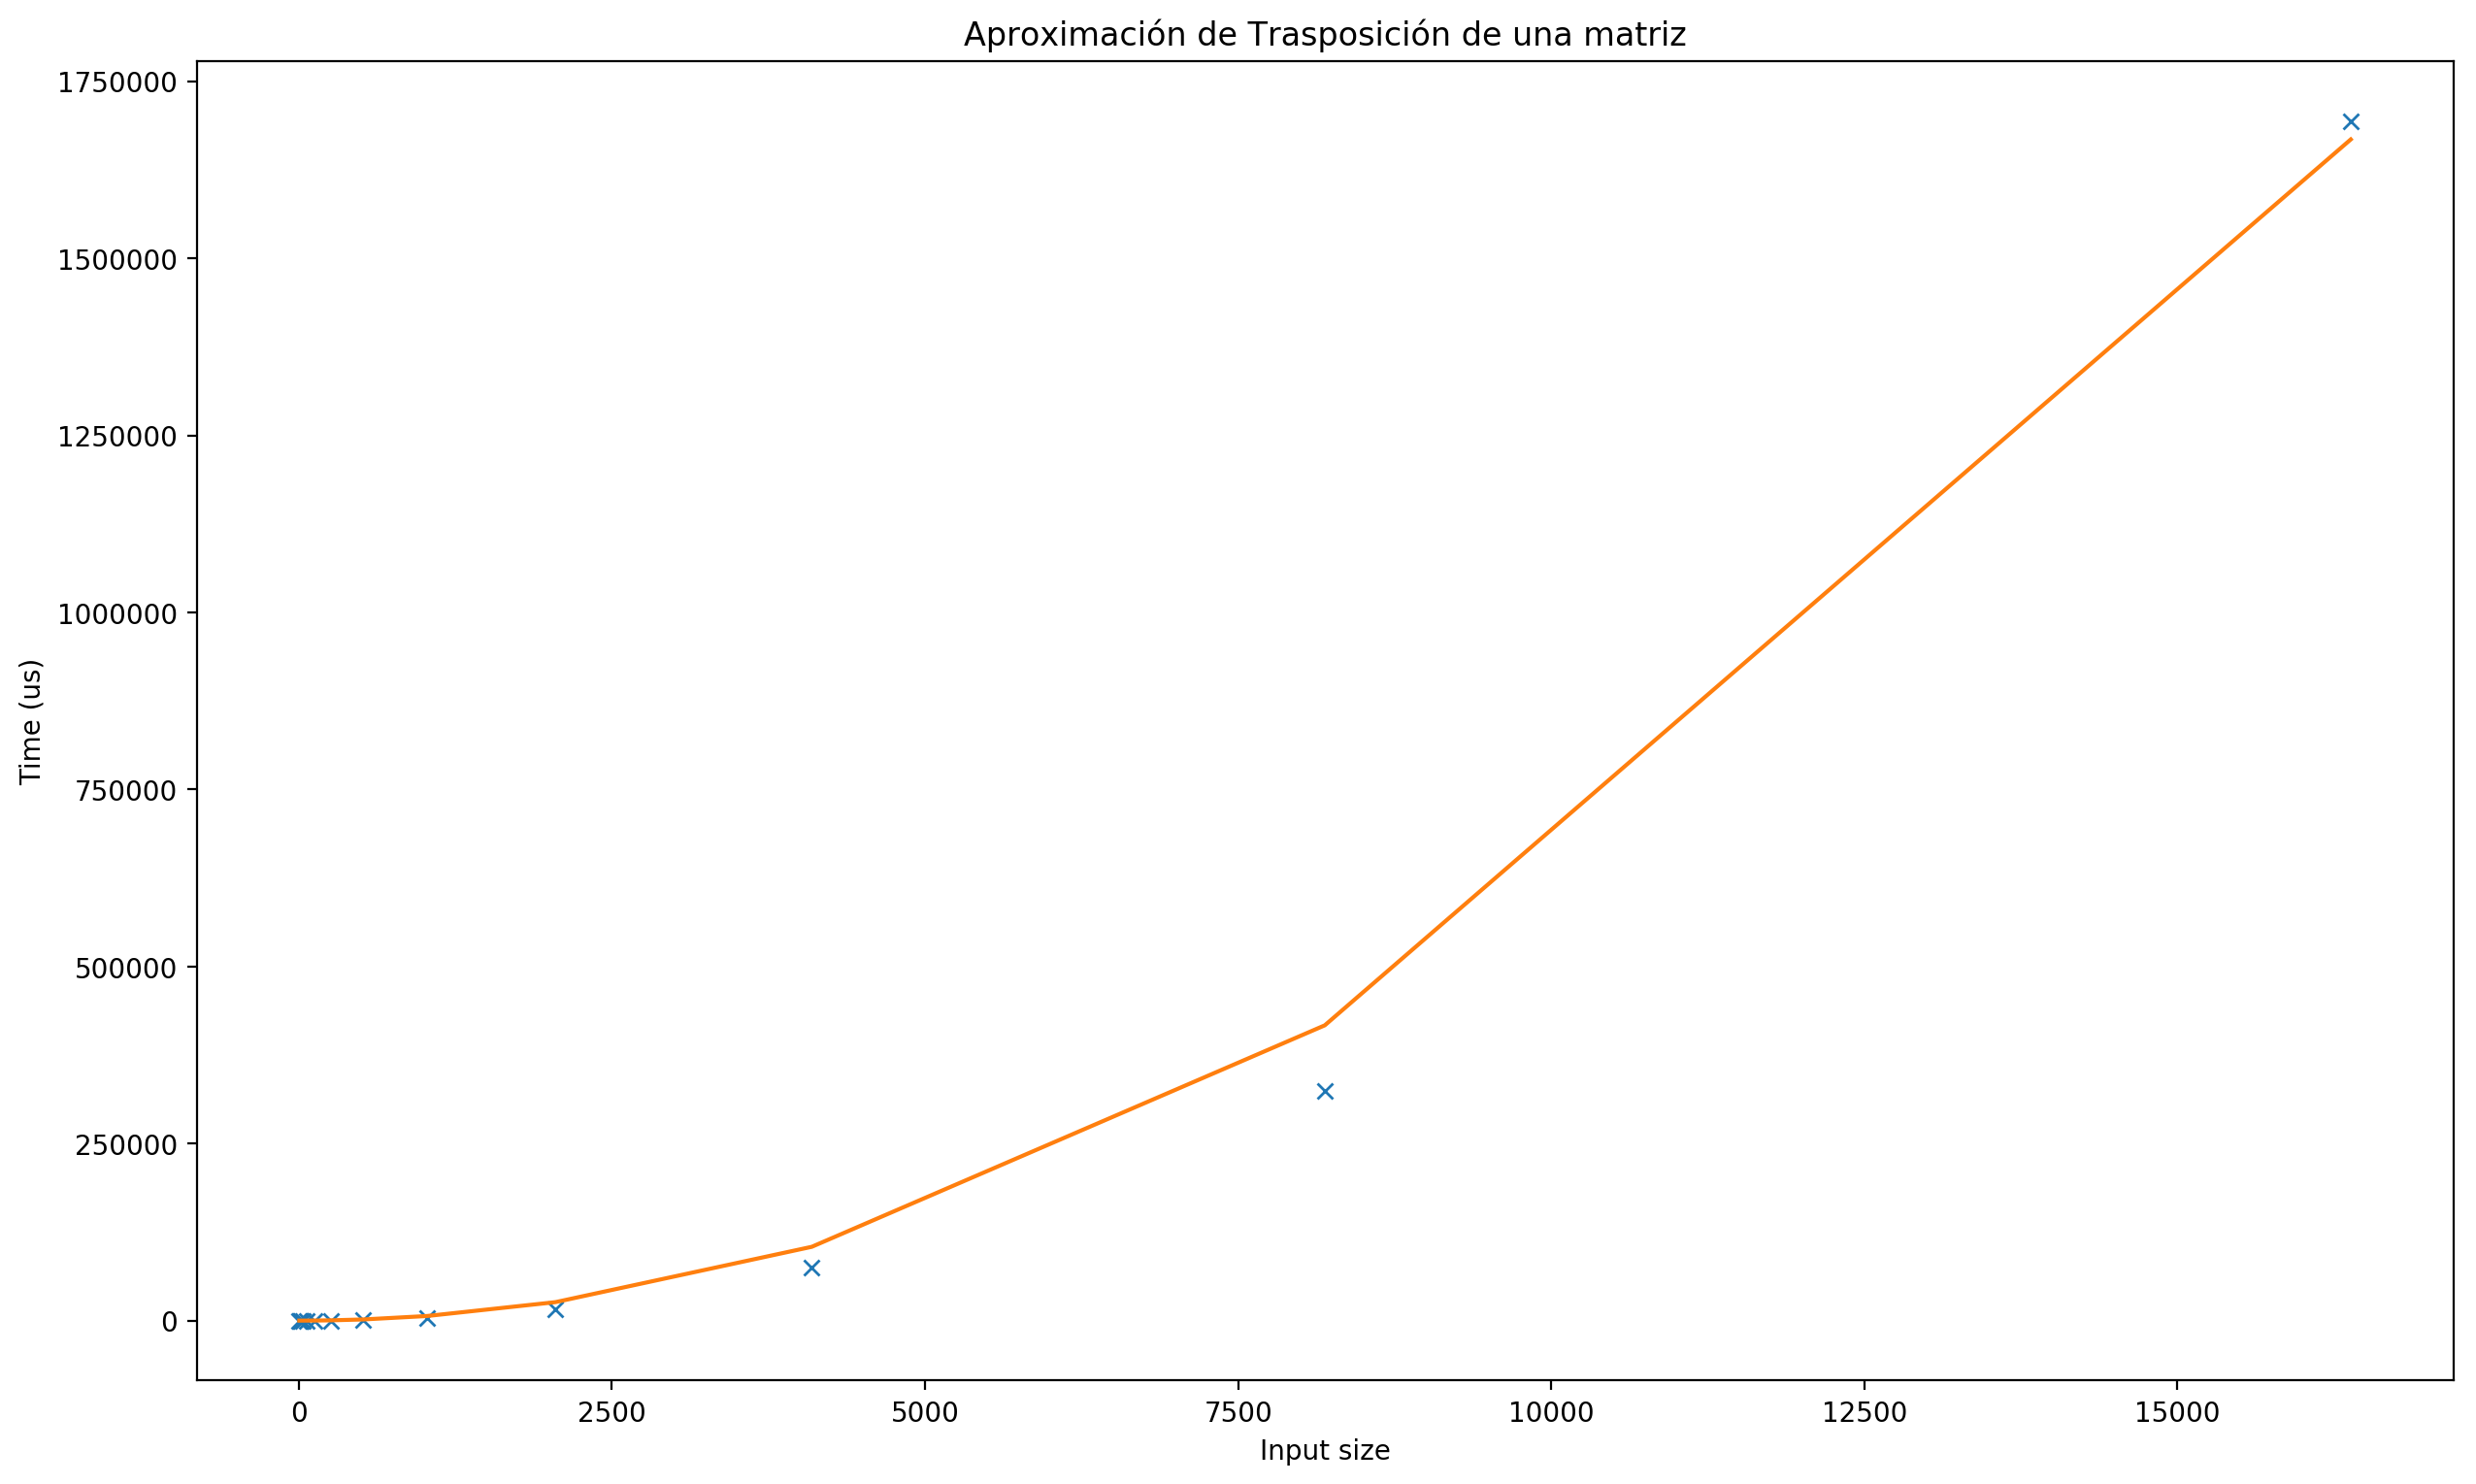
\includegraphics[width=\textwidth]{./Graficas/trasponer_iter_funcion.png}
\end{frame}

\begin{frame}[fragile]{Traspuesta de una matriz}
\begin{lstlisting}[language=C]
void trasponerRec(int **mat, int inicio_c, int fin_c, int fila) {
    if ( fin_c - inicio_c > 1 ) {
        int aux;

        for ( int i = fila; i < fila + (fin_c - inicio_c)/2; i++ ) {
            for ( int j = inicio_c + (fin_c - inicio_c)/2; j < fin_c; j++ ) {
                aux = mat[i + (fin_c - inicio_c)/2][j-(fin_c - inicio_c)/2];
                mat[i + (fin_c - inicio_c)/2][j-(fin_c - inicio_c)/2] = mat[i][j];
                mat[i][j] = aux;
            }
        }

        trasponerRec(mat, inicio_c, inicio_c+(fin_c-inicio_c)/2, fila);
        trasponerRec(mat, inicio_c+(fin_c-inicio_c)/2, fin_c, fila);
        trasponerRec(mat, inicio_c, inicio_c+(fin_c-inicio_c)/2, fila+(fin_c-inicio_c)/2);
        trasponerRec(mat, inicio_c+(fin_c-inicio_c)/2, fin_c, fila+(fin_c-inicio_c)/2);
    }
}

void trasponer(int **mat, int tam) {
    trasponerRec(mat, 0, tam, 0);
}
\end{lstlisting}
\end{frame}
\begin{frame}[fragile]{Traspuesta de una matriz}
\begin{lstlisting}[language=C]
void trasponerRec(int **mat, int inicio_c, int fin_c, int fila) {
...

	trasponerRec(mat, inicio_c, inicio_c+(fin_c-inicio_c)/2, fila);
	trasponerRec(mat, inicio_c+(fin_c-inicio_c)/2, fin_c, fila);
	trasponerRec(mat, inicio_c, inicio_c+(fin_c-inicio_c)/2, fila+(fin_c-inicio_c)/2);
	trasponerRec(mat, inicio_c+(fin_c-inicio_c)/2, fin_c, fila+(fin_c-inicio_c)/2);
}
}

void trasponer(int **mat, int tam) {
	trasponerRec(mat, 0, tam, 0);
}
\end{lstlisting}
\end{frame}

\begin{frame}[fragile]{Traspuesta de una matriz. \normalfont{Eficiencia teórica}}

Primero vamos a calcular la eficiencia de los dos for anidados:

Podemos ver que el for interno tiene una eficiencia de:  $$\sum_{inicio_c+\frac{fin\_c-inicio\_c}{2}}^{fin\_c-1} 1 = fin\_c-1 - (inicio\_c+\frac{fin\_c-inicio\_c}{2})+1 = \frac{fin\_c-inicio\_c}{2}$$

Llamaremos $$n=\frac{fin\_c-inicio\_c}{2}$$
\end{frame}

\begin{frame}[fragile]{Traspuesta de una matriz. \normalfont{Eficiencia teórica}}
Eficiencia del for externo:
$$\sum_{fila}^{fila+n-1}n= n·(fila+n-1-fila+1) = n ^ 2$$

Obtenemos así la ecuación de recurrencia: $$T(n) = n^2 +4T(n/2)$$
\end{frame}

\begin{frame}[fragile]{Traspuesta de una matriz. \normalfont{Eficiencia teórica}}
$$T(n) = n^2 +4T(n/2)$$
$$T(2^k) = (2^k)^2+4T(2^{k-1})$$
$$T(2^k)-4T(2^{k-1}) = 4^k$$
$$(x-4)(x-4) = 0; (x-4)^2$$
$$T_k = c_1*4^k+c_2*k*4^k$$
$$T_n = 2*c_1*n^2 + 2*c_2*n^2\log(n)$$
Por lo que $$T(n) \in O(n^2\log (n))$$
\end{frame}




\begin{frame}[fragile]{Traspuesta de una matriz. \normalfont{Eficiencia empírica}}
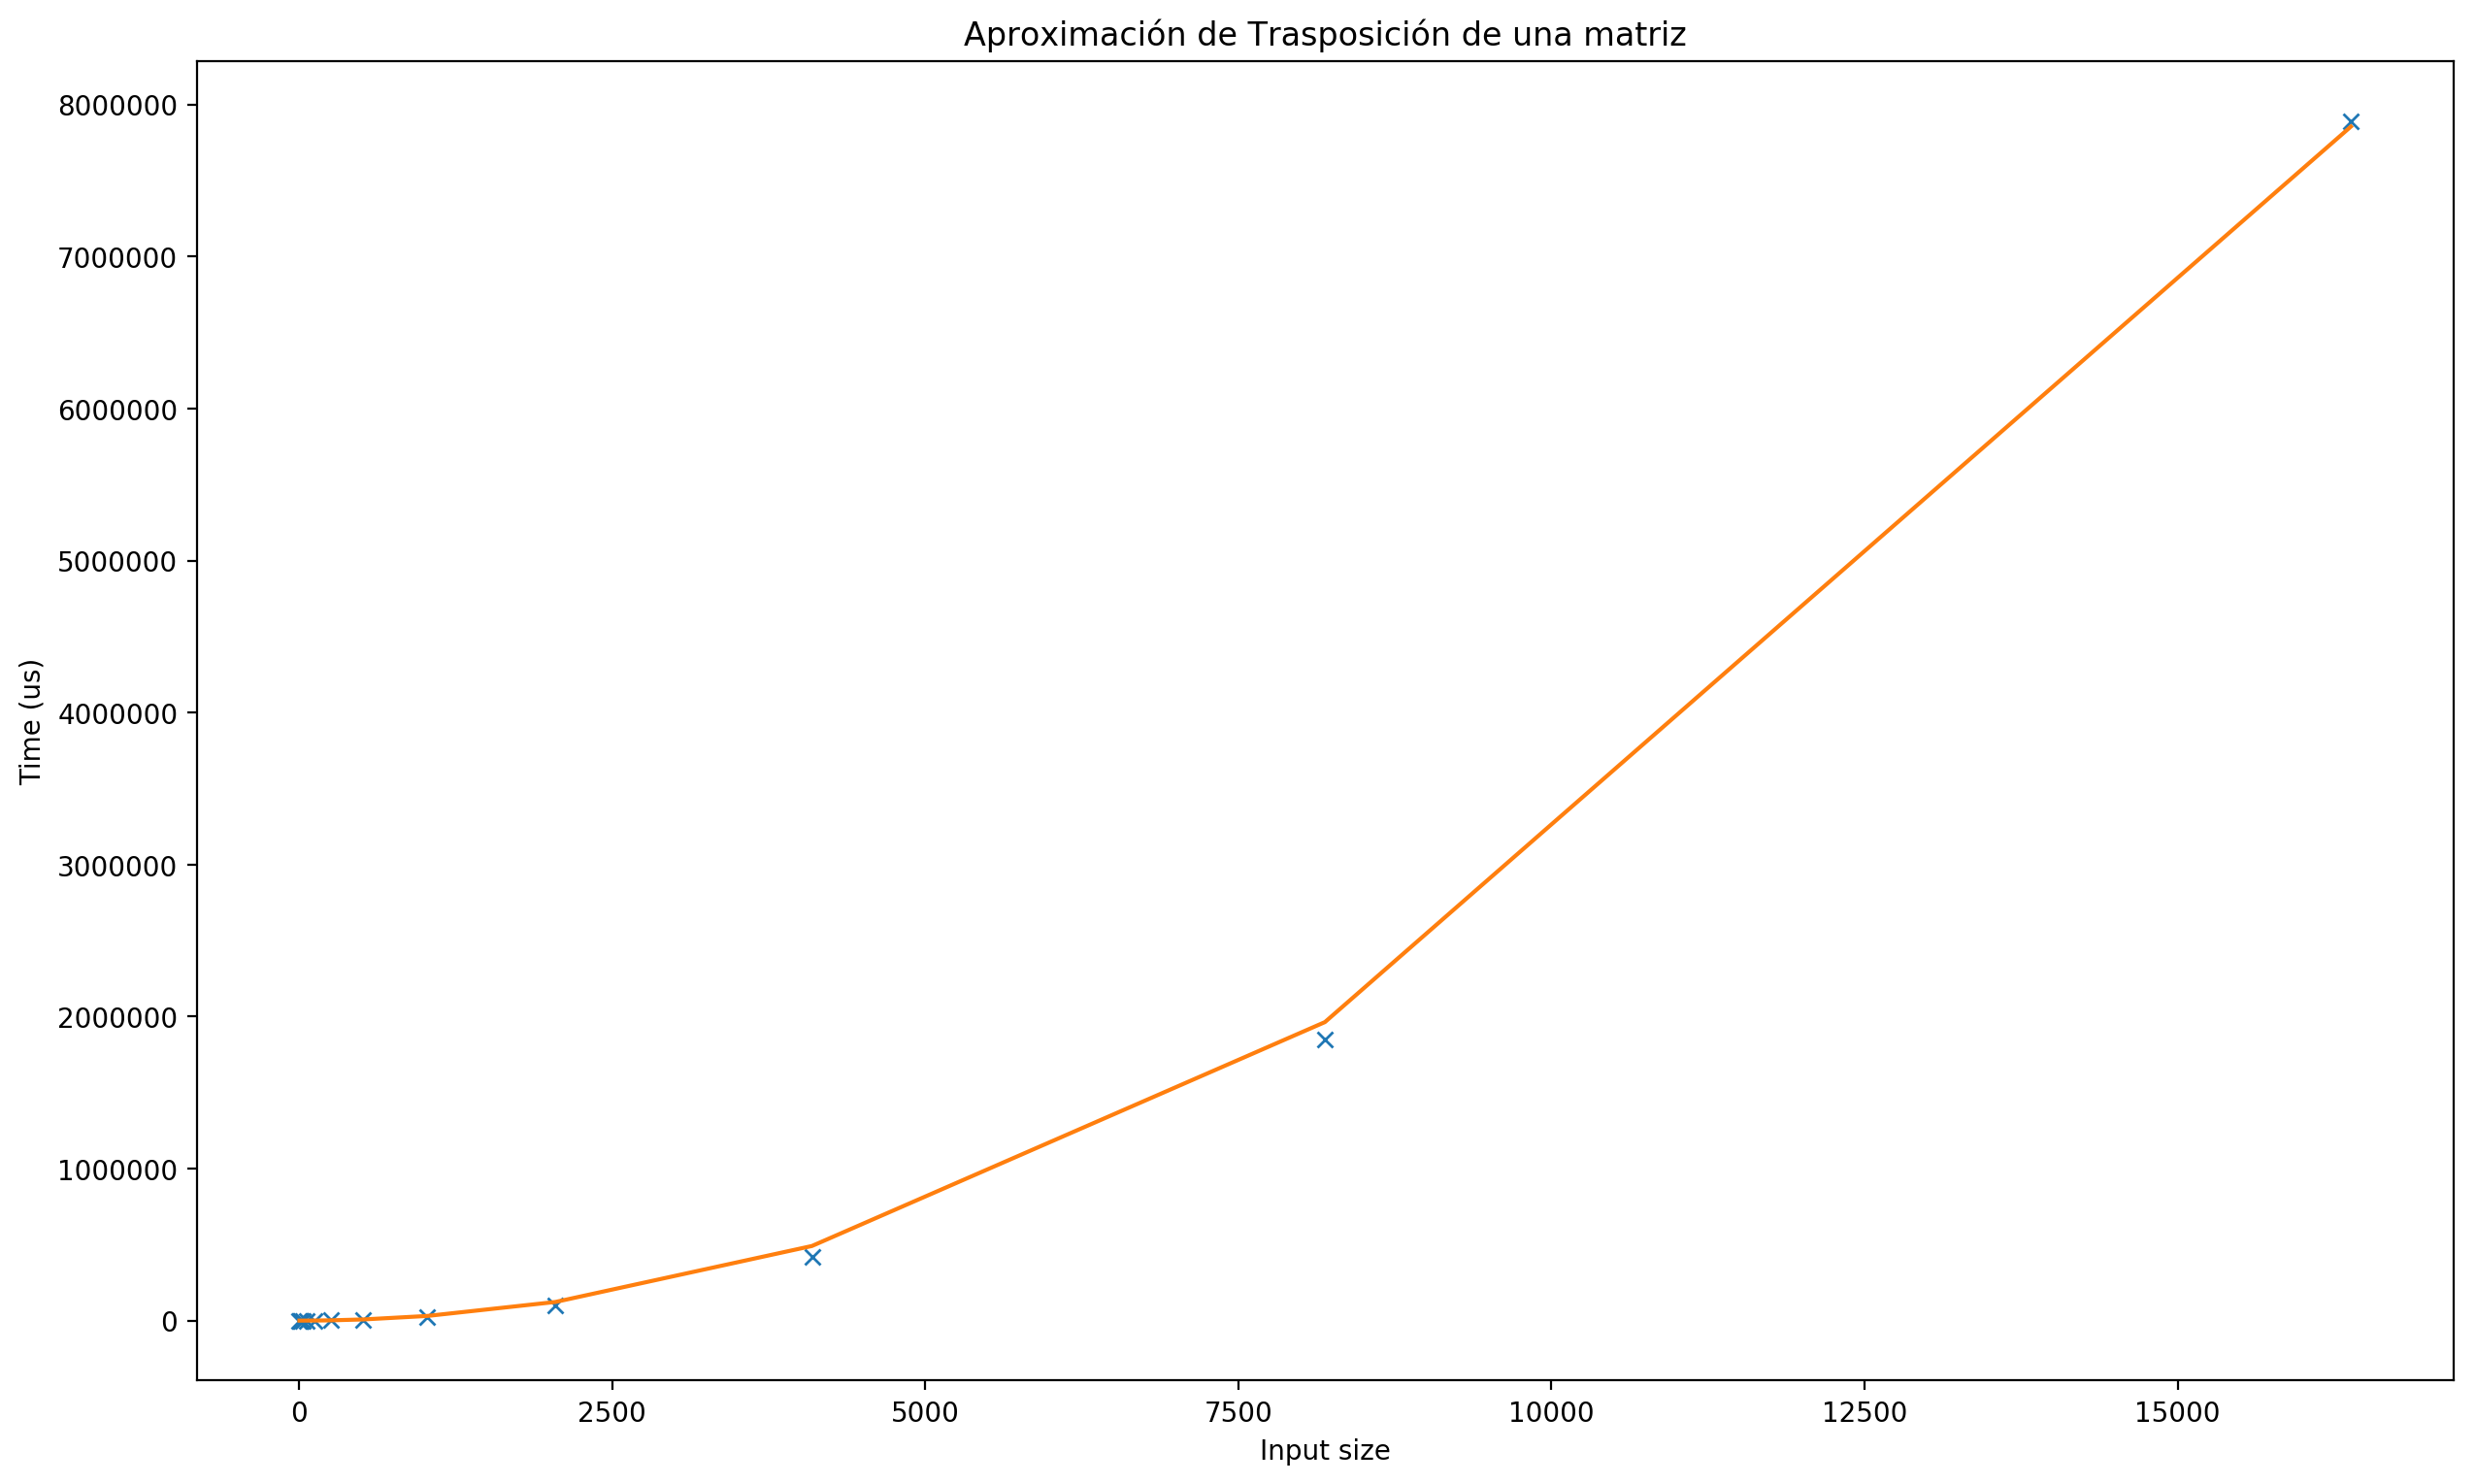
\includegraphics[width=\textwidth]{./Graficas/trasponer_div_funcion.png}
\end{frame}

\begin{frame}[fragile]{Traspuesta de una matriz. \normalfont{Gráfica ambos}}
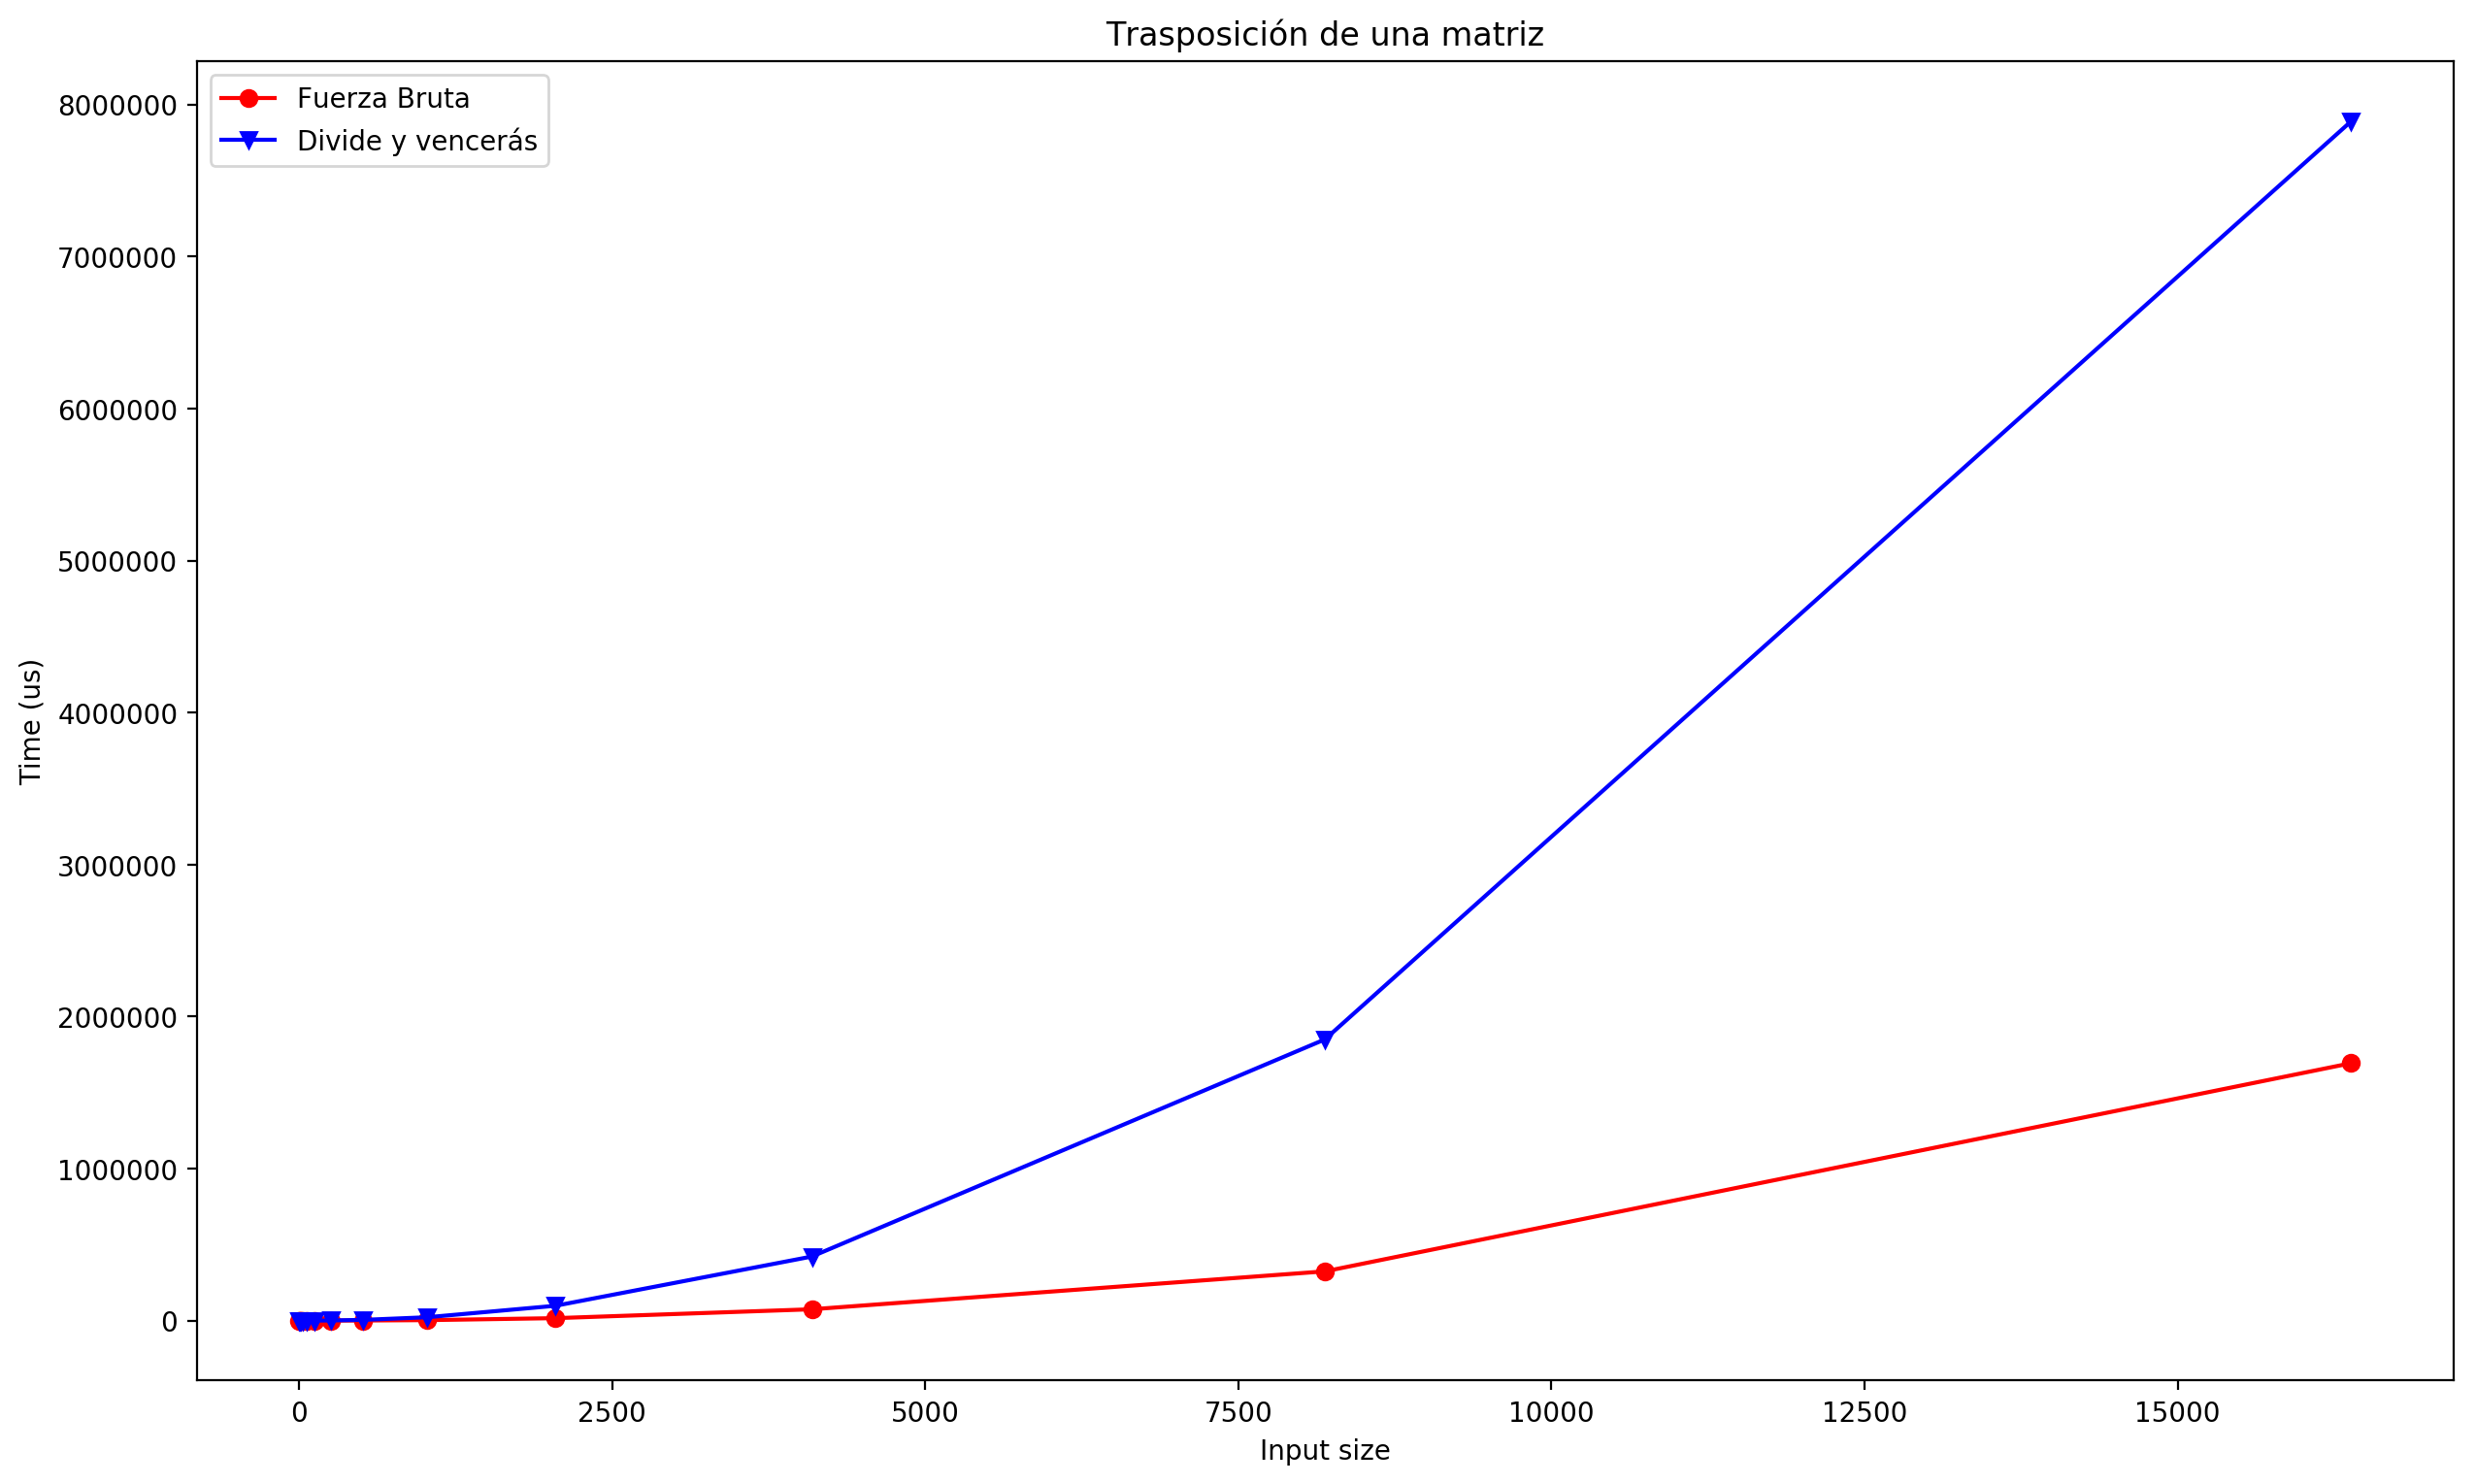
\includegraphics[width=\textwidth]{./Graficas/trasponer_ambos.png}
\end{frame}



\begin{frame}[fragile]{Mezclar \textit{k} vectores ordenados (sin DyV)}
\begin{lstlisting}[language=C]
vector<vector<int> > merge_first_two_vectors(vector<vector<int> > matrix){
	// Matriz con un vector menos, resultado de la mezcla
	vector<vector<int> > merged_matrix(matrix.size() - 1);

	// Vector que hemos mezclado
	vector<int> merged = merge(matrix[0], matrix[1]);
	
	// Calculamos los datos de la nueva matriz
	merged_matrix[0] = merged;
	for(int i = 1; i < merged_matrix.size(); i++){
		merged_matrix[i] = matrix[i+1];
	}
	
	return merged_matrix;
}
\end{lstlisting}
\end{frame}

\begin{frame}[fragile]{Mezclar \textit{k} vectores ordenados (sin DyV)}
\begin{lstlisting}[language=C]
vector<int> merge_vectors_basic(vector<vector<int> > matrix){
	// Caso base para parar la recursividad
	if(matrix.size() == 1){
		return parse_matrix_to_vector(matrix);	
	}else{
		matrix = merge_first_two_vectors(matrix);
		return merge_vectors_basic(matrix);
	}
}

\end{lstlisting}
\end{frame}

\begin{frame}[fragile]{Mezclar \textit{k} vectores ordenados. \normalfont{Eficiencia teórica (sin DyV)}}
\begin{center}
	\textbf{\large{\texttt{merge}}}
\end{center}

En el peor de los casos el algoritmo recorre los dos vectores, el tiempo va a ser $2k$, que es una constante, por lo que: $$T(n) \in O(1)$$
\end{frame}

\begin{frame}[fragile]{Mezclar \textit{k} vectores ordenados (sin DyV). \normalfont{Eficiencia teórica}}

\begin{center}
	\textbf{\large{\texttt{merge\_first\_two\_vectors}}}
\end{center}

En la primera parte del código destaca la llamada a la función \texttt{merge}, que como hemos calculado anteriormente es $O(1)$, el bucle for también es $O(n)$, por lo que 
$$T(n) \in O(n)$$

\end{frame}

\begin{frame}[fragile]{Mezclar \textit{k} vectores ordenados (sin DyV). \normalfont{Eficiencia teórica}}
\begin{center}
	\textbf{\large{\texttt{merge\_vectors\_basic}}}
\end{center}

Podemos observar que el algoritmo hace $(n-1)$ veces la función \texttt{merge\_first\_two\_vectors} por lo que $T(n) = (n-1)*n$. 

Concluimos así que
$$T(n) \in O(n^2)$$

\end{frame}



\begin{frame}[fragile]{Mezclar \textit{k} vectores ordenados (sin DyV). \normalfont{Eficiencia empírica}}
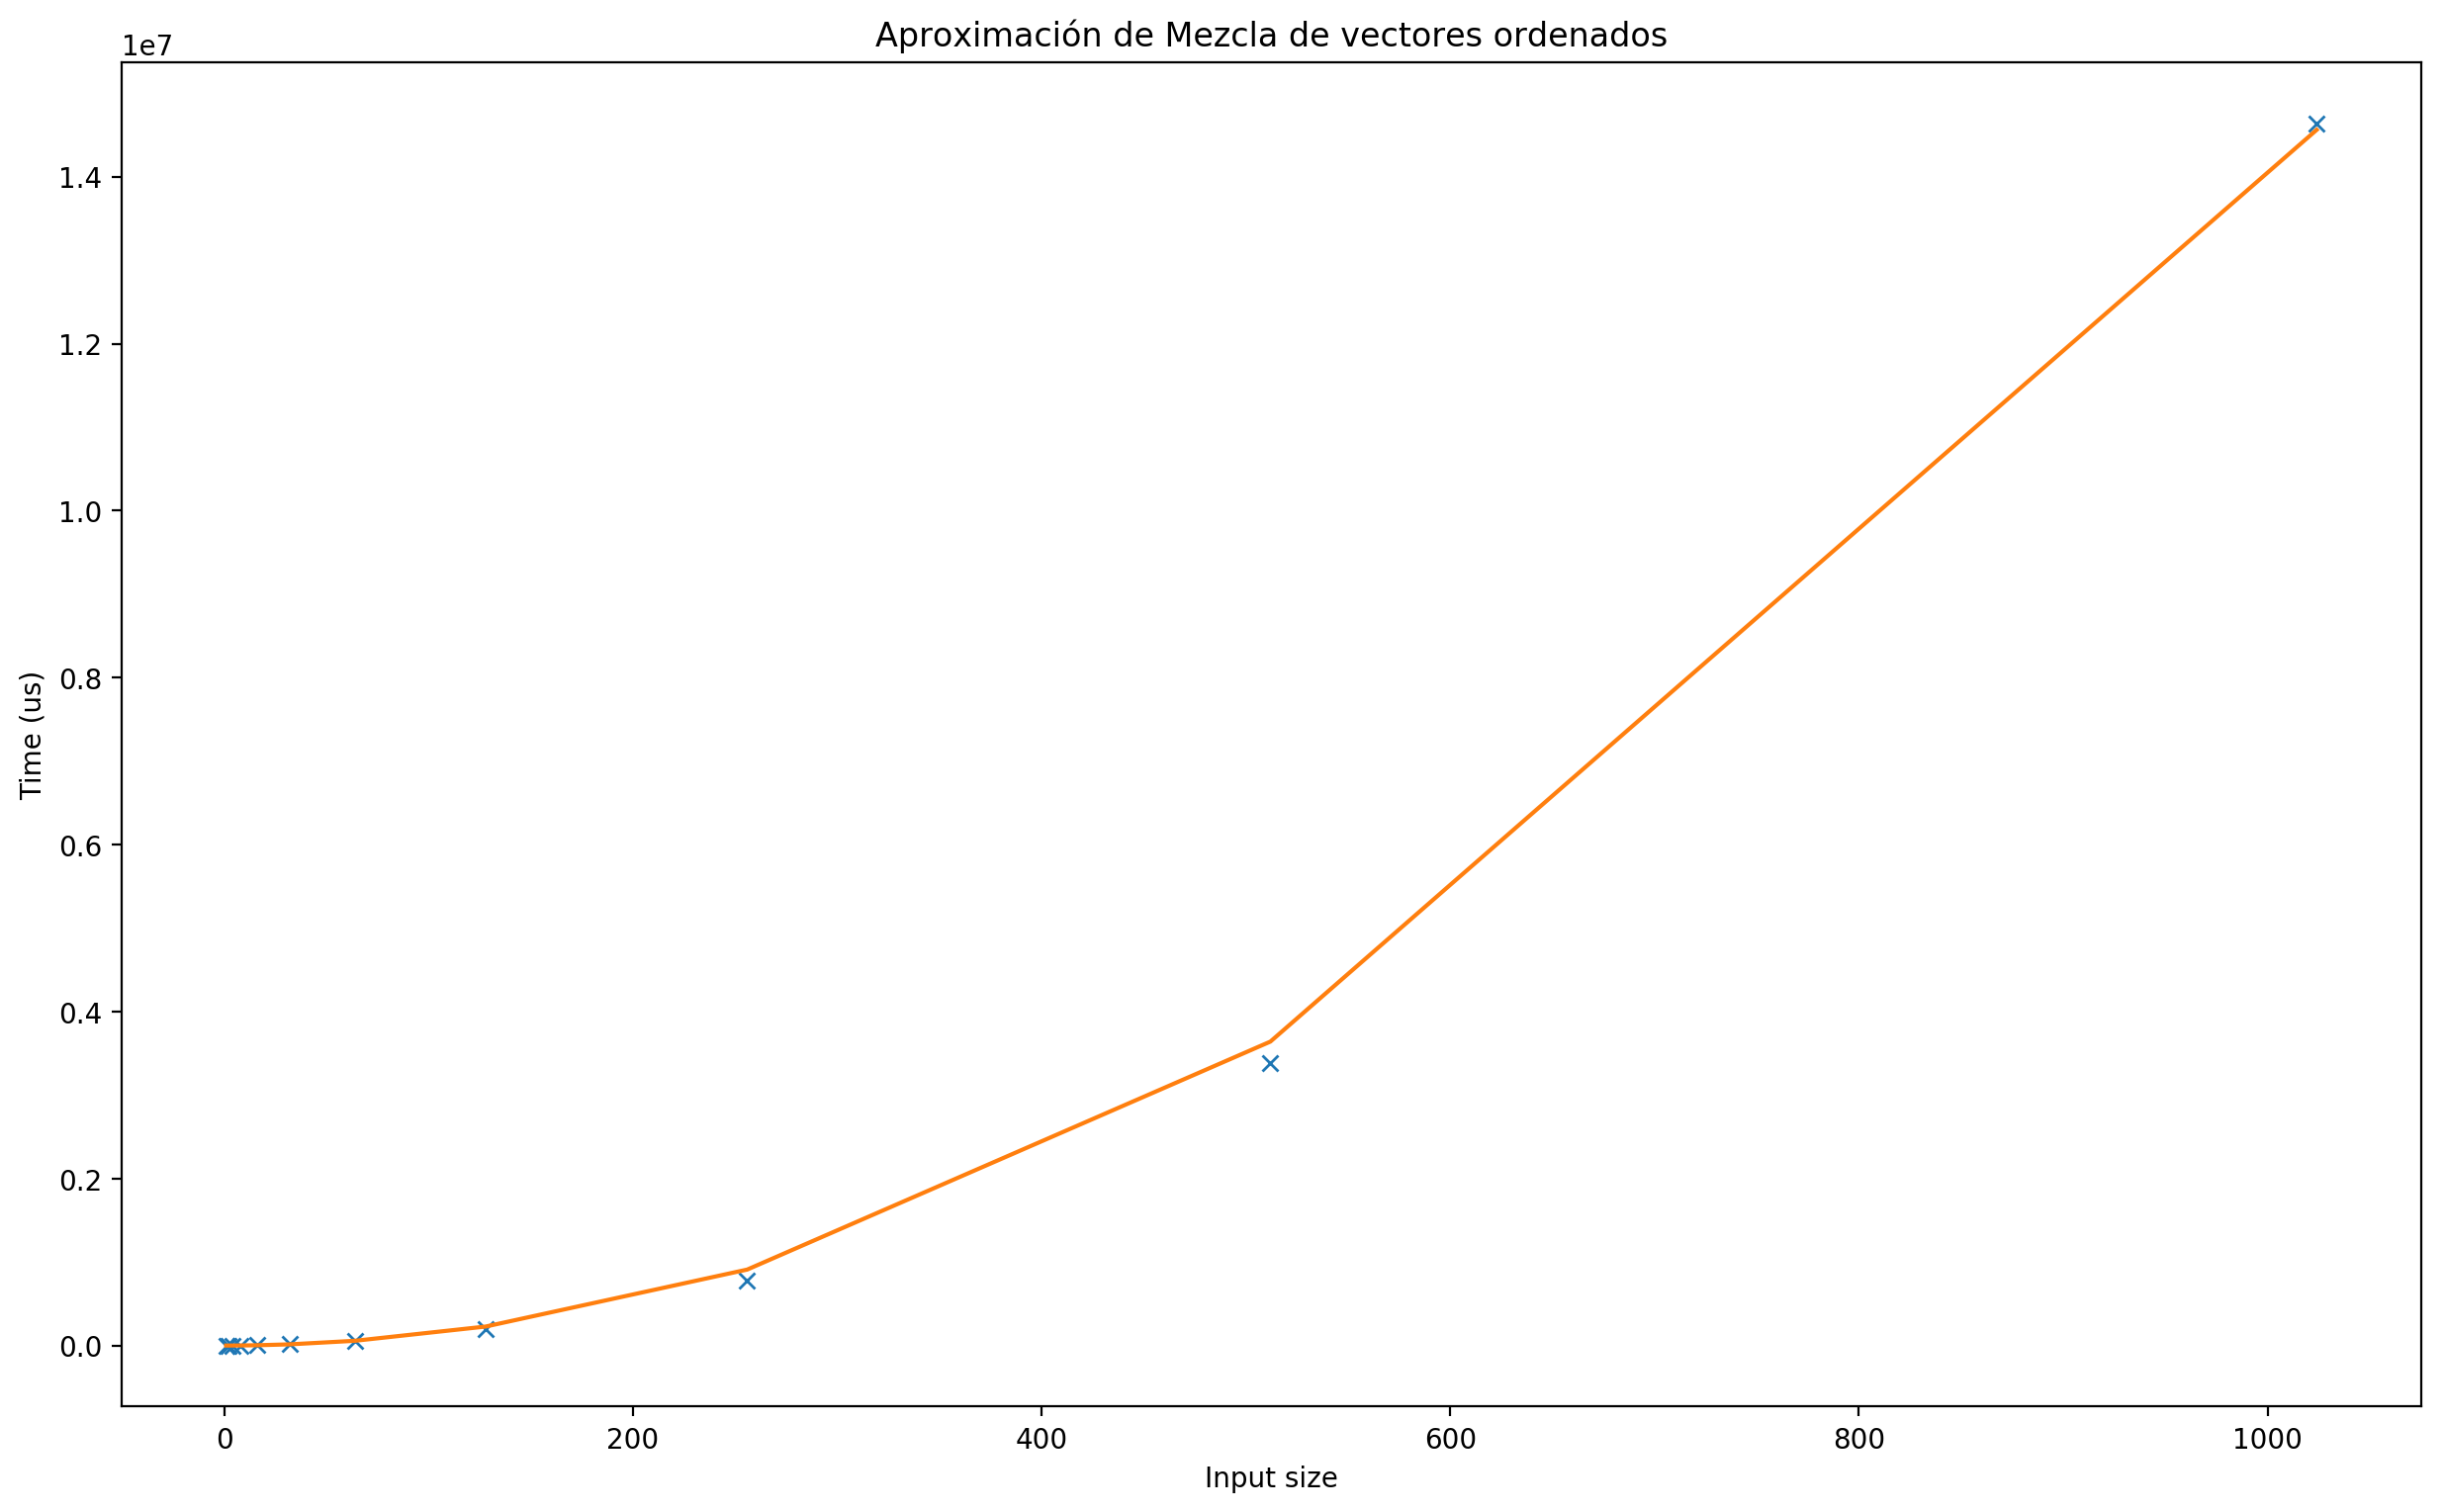
\includegraphics[width=\textwidth]{./Graficas/merge_iter_funcion.png}
\end{frame}

\begin{frame}[fragile]{Mezclar \textit{k} vectores ordenados}
\begin{lstlisting}[language=C]
vector<int> merge(vector<int> v1, vector<int> v2){
	vector<int> merged(v1.size() + v2.size());
	int pos1 = 0, pos2 = 0;
	
	while(pos1 < v1.size() || pos2 < v2.size()){
		if(pos1 == v1.size()){
			merged[pos1 + pos2] = v2[pos2]; pos2++;
		}else if(pos2 == v2.size()){
			merged[pos1 + pos2] = v1[pos1];	pos1++;
		}else{
			if(v1[pos1] < v2[pos2]){
				merged[pos1 + pos2] = v1[pos1]; pos1++;
			}else{
				merged[pos1 + pos2] = v2[pos2]; pos2++;
			}
		}
	}
	return merged;
}

\end{lstlisting}
\end{frame}
\begin{frame}[fragile]{Mezclar \textit{k} vectores ordenados}
\begin{lstlisting}[language=C]
vector<vector<int> > merge_two_by_two(vector<vector<int> > matrix){
	// Generamos la nueva matriz
	int new_size = (matrix.size() / 2) + matrix.size() % 2;
	vector<vector<int> > merged_matrix(new_size);
	
	// Tomamos los datos de la nueva matriz
	for(int i = 0; i < merged_matrix.size(); i++){
		// Ultimo elemento de la matriz sin hacer merge
		if(2*i + 1 >= matrix.size()){
			merged_matrix[i] = merged_matrix[2*i + 1];
		}
	
		vector<int> new_vector = merge(matrix[2*i], matrix[2*i + 1]);
		merged_matrix[i] = new_vector;
	}
	
	return merged_matrix;
}


\end{lstlisting}
\end{frame}

\begin{frame}[fragile]{Mezclar \textit{k} vectores ordenados}
\begin{lstlisting}[language=C]
vector<int> merge_divide_and_conquer(vector<vector<int> > matrix){
	// Caso base para finalizar la recursividad
	if(matrix.size() == 1){
		return parse_matrix_to_vector(matrix);
	}

	// Reduzco el tamaño del problema a la mitad y aplico recursividad
	matrix = merge_two_by_two(matrix);
	return merge_divide_and_conquer(matrix);
}

\end{lstlisting}
\end{frame}


\begin{frame}[fragile]{Mezclar \textit{k} vectores ordenados. \normalfont{Eficiencia teórica}}
\begin{center}
\textbf{\large{\texttt{merge\_two\_by\_two}}}
\end{center}
Podemos ver que el tamaño del vector se divide en dos, y luego el for hace $\frac{n}{2}k$ iteraciones, por lo que 
$$T(n) \in O(n)$$ 
\end{frame}
\begin{frame}[fragile]{Mezclar \textit{k} vectores ordenados. \normalfont{Eficiencia teórica}}
\begin{center}
\textbf{\large{\texttt{merge\_divide\_and\_conquer}}}
\end{center}

$$T(n)=T(\frac{n}{2})+\frac{n}{2}*k +1 $$
$$T(n) = T(\frac{n}{2}) + nk +1$$
$$T(2^m) - T(2^{m-1}) = 2^mk+1$$
$$(x-1)^2(x-2) = 0$$
$$T_m = c_1 + c_2m +c_32^m$$
$$T_n = c_1 + c_2log(n) + c_3n$$
Por lo que:
$$T(n) \in O(n)$$
\end{frame}


\begin{frame}[fragile]{Mezclar \textit{k} vectores ordenados. \normalfont{Eficiencia empírica}}
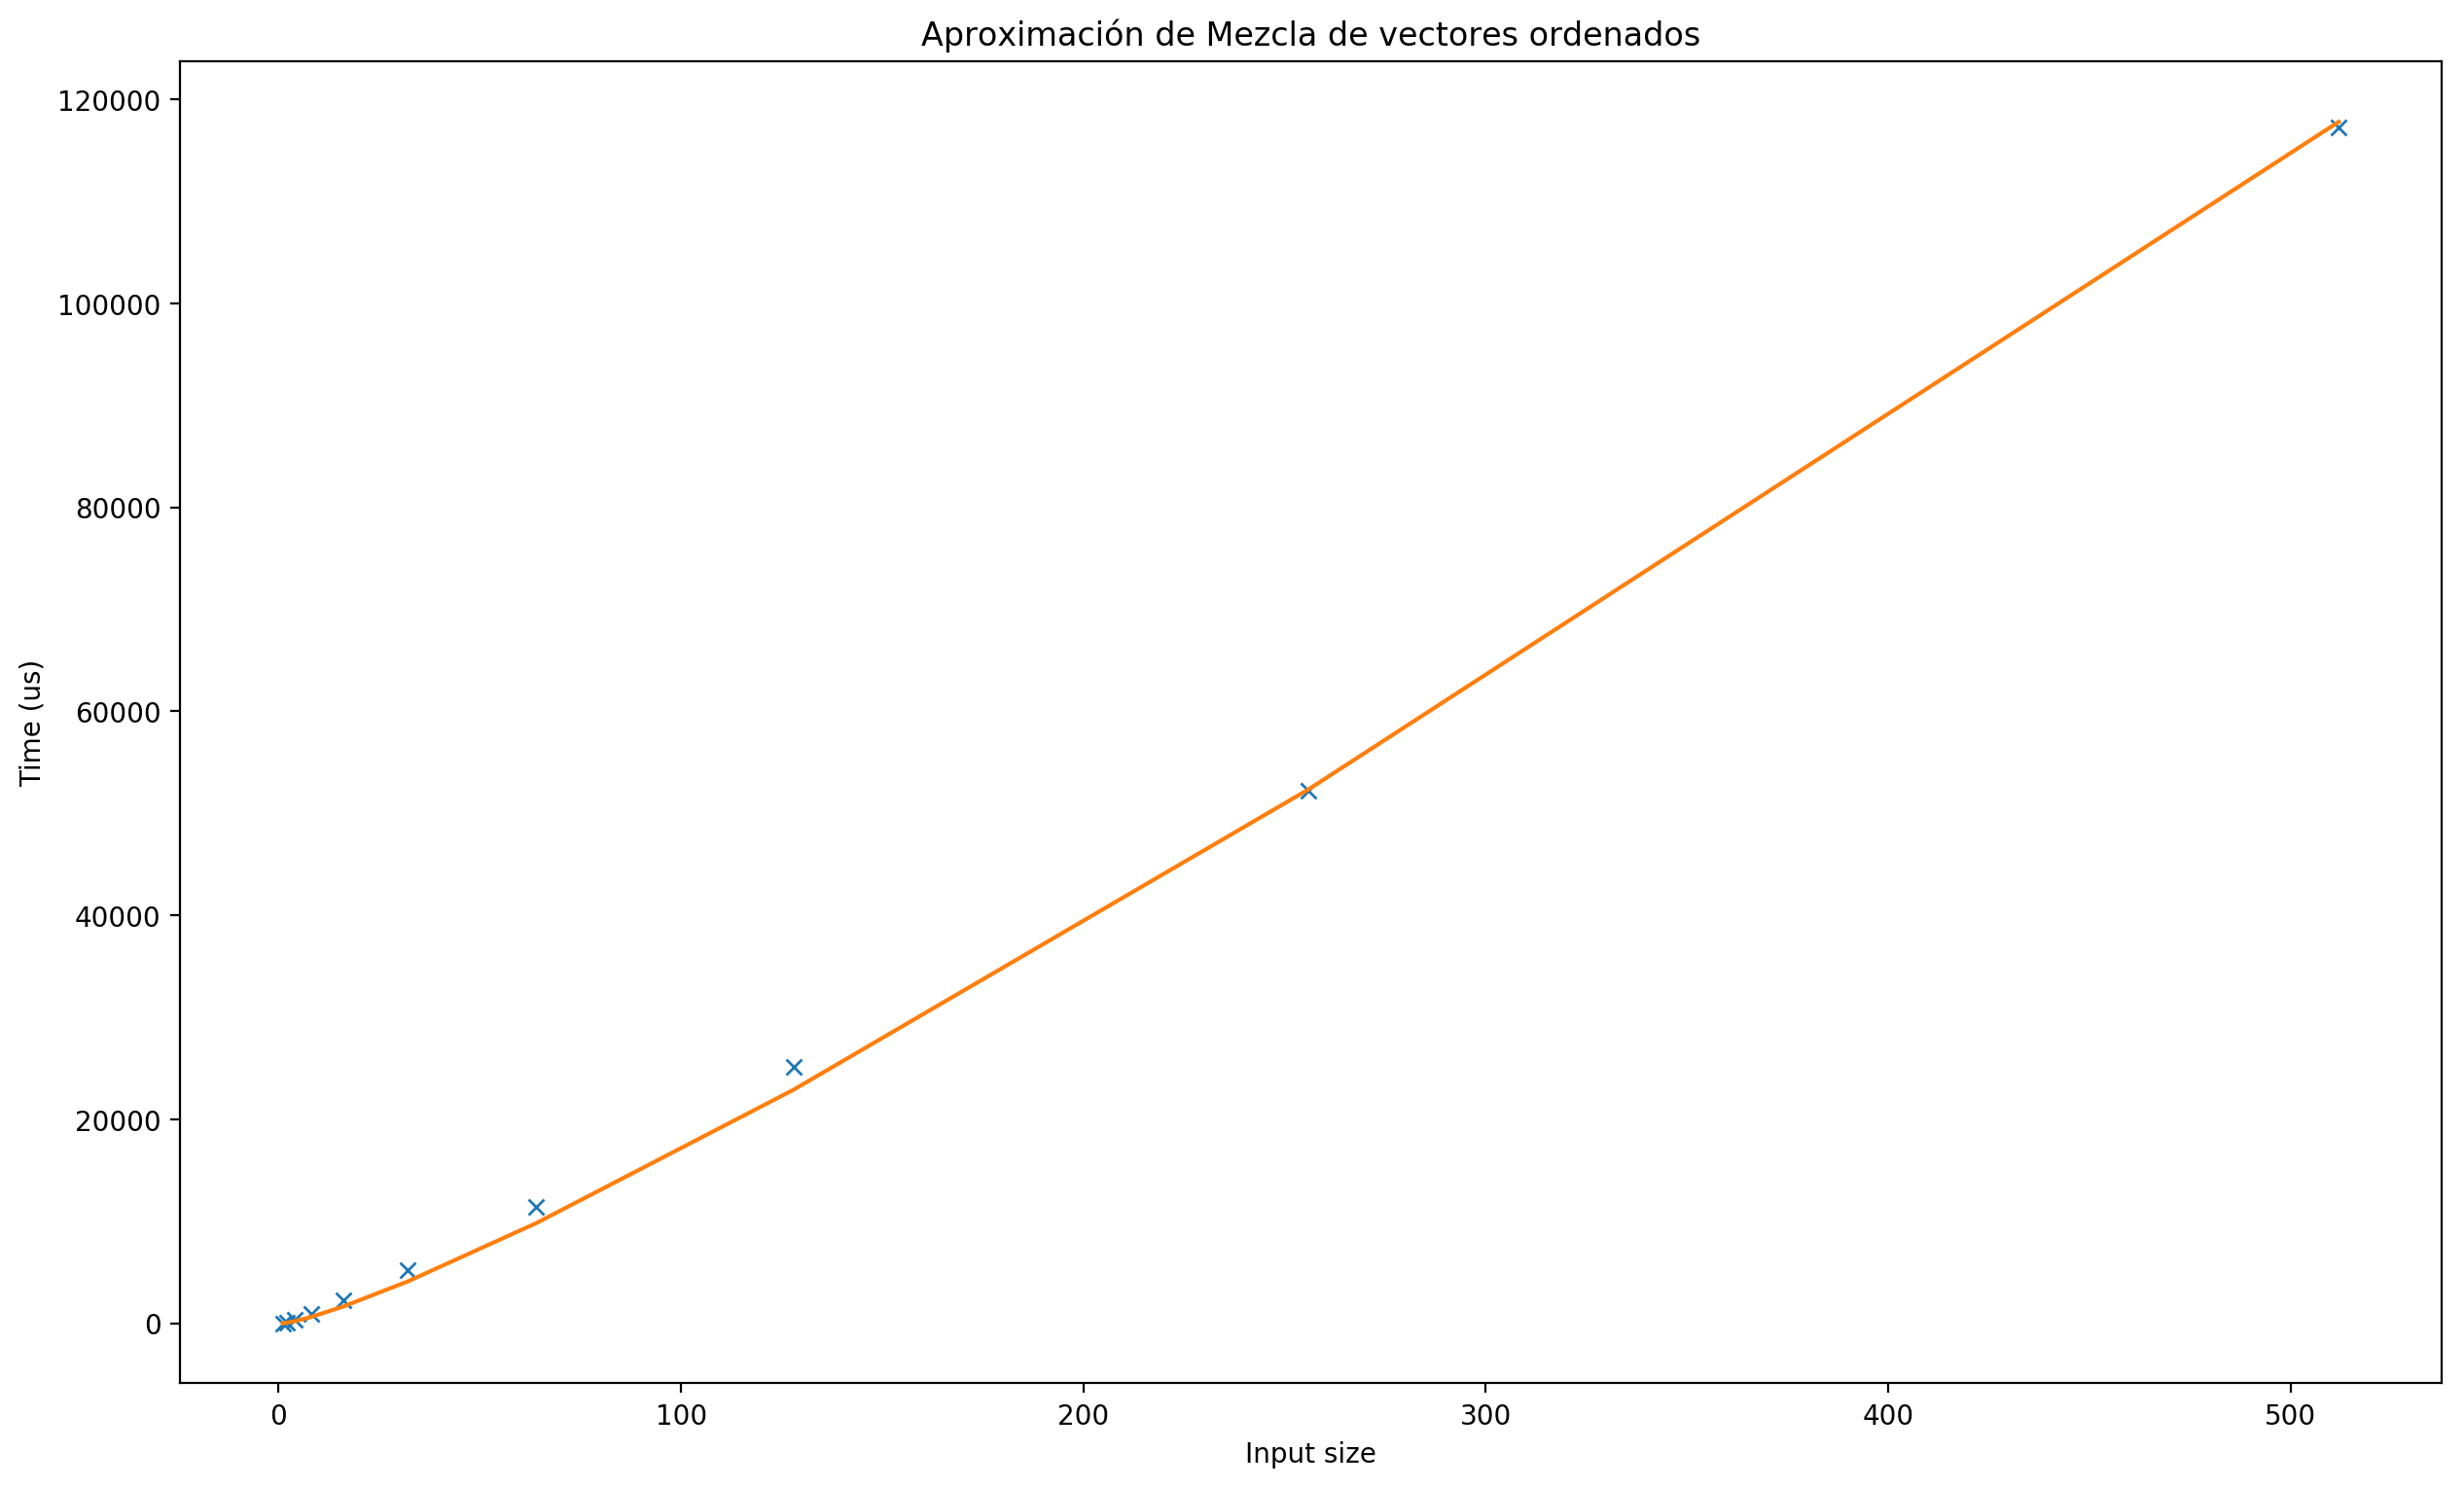
\includegraphics[width=\textwidth]{./Graficas/merge_div_funcion.png}
\end{frame}

\begin{frame}[fragile]{Mezclar \textit{k} vectores ordenados. \normalfont{Gráfica ambos}}
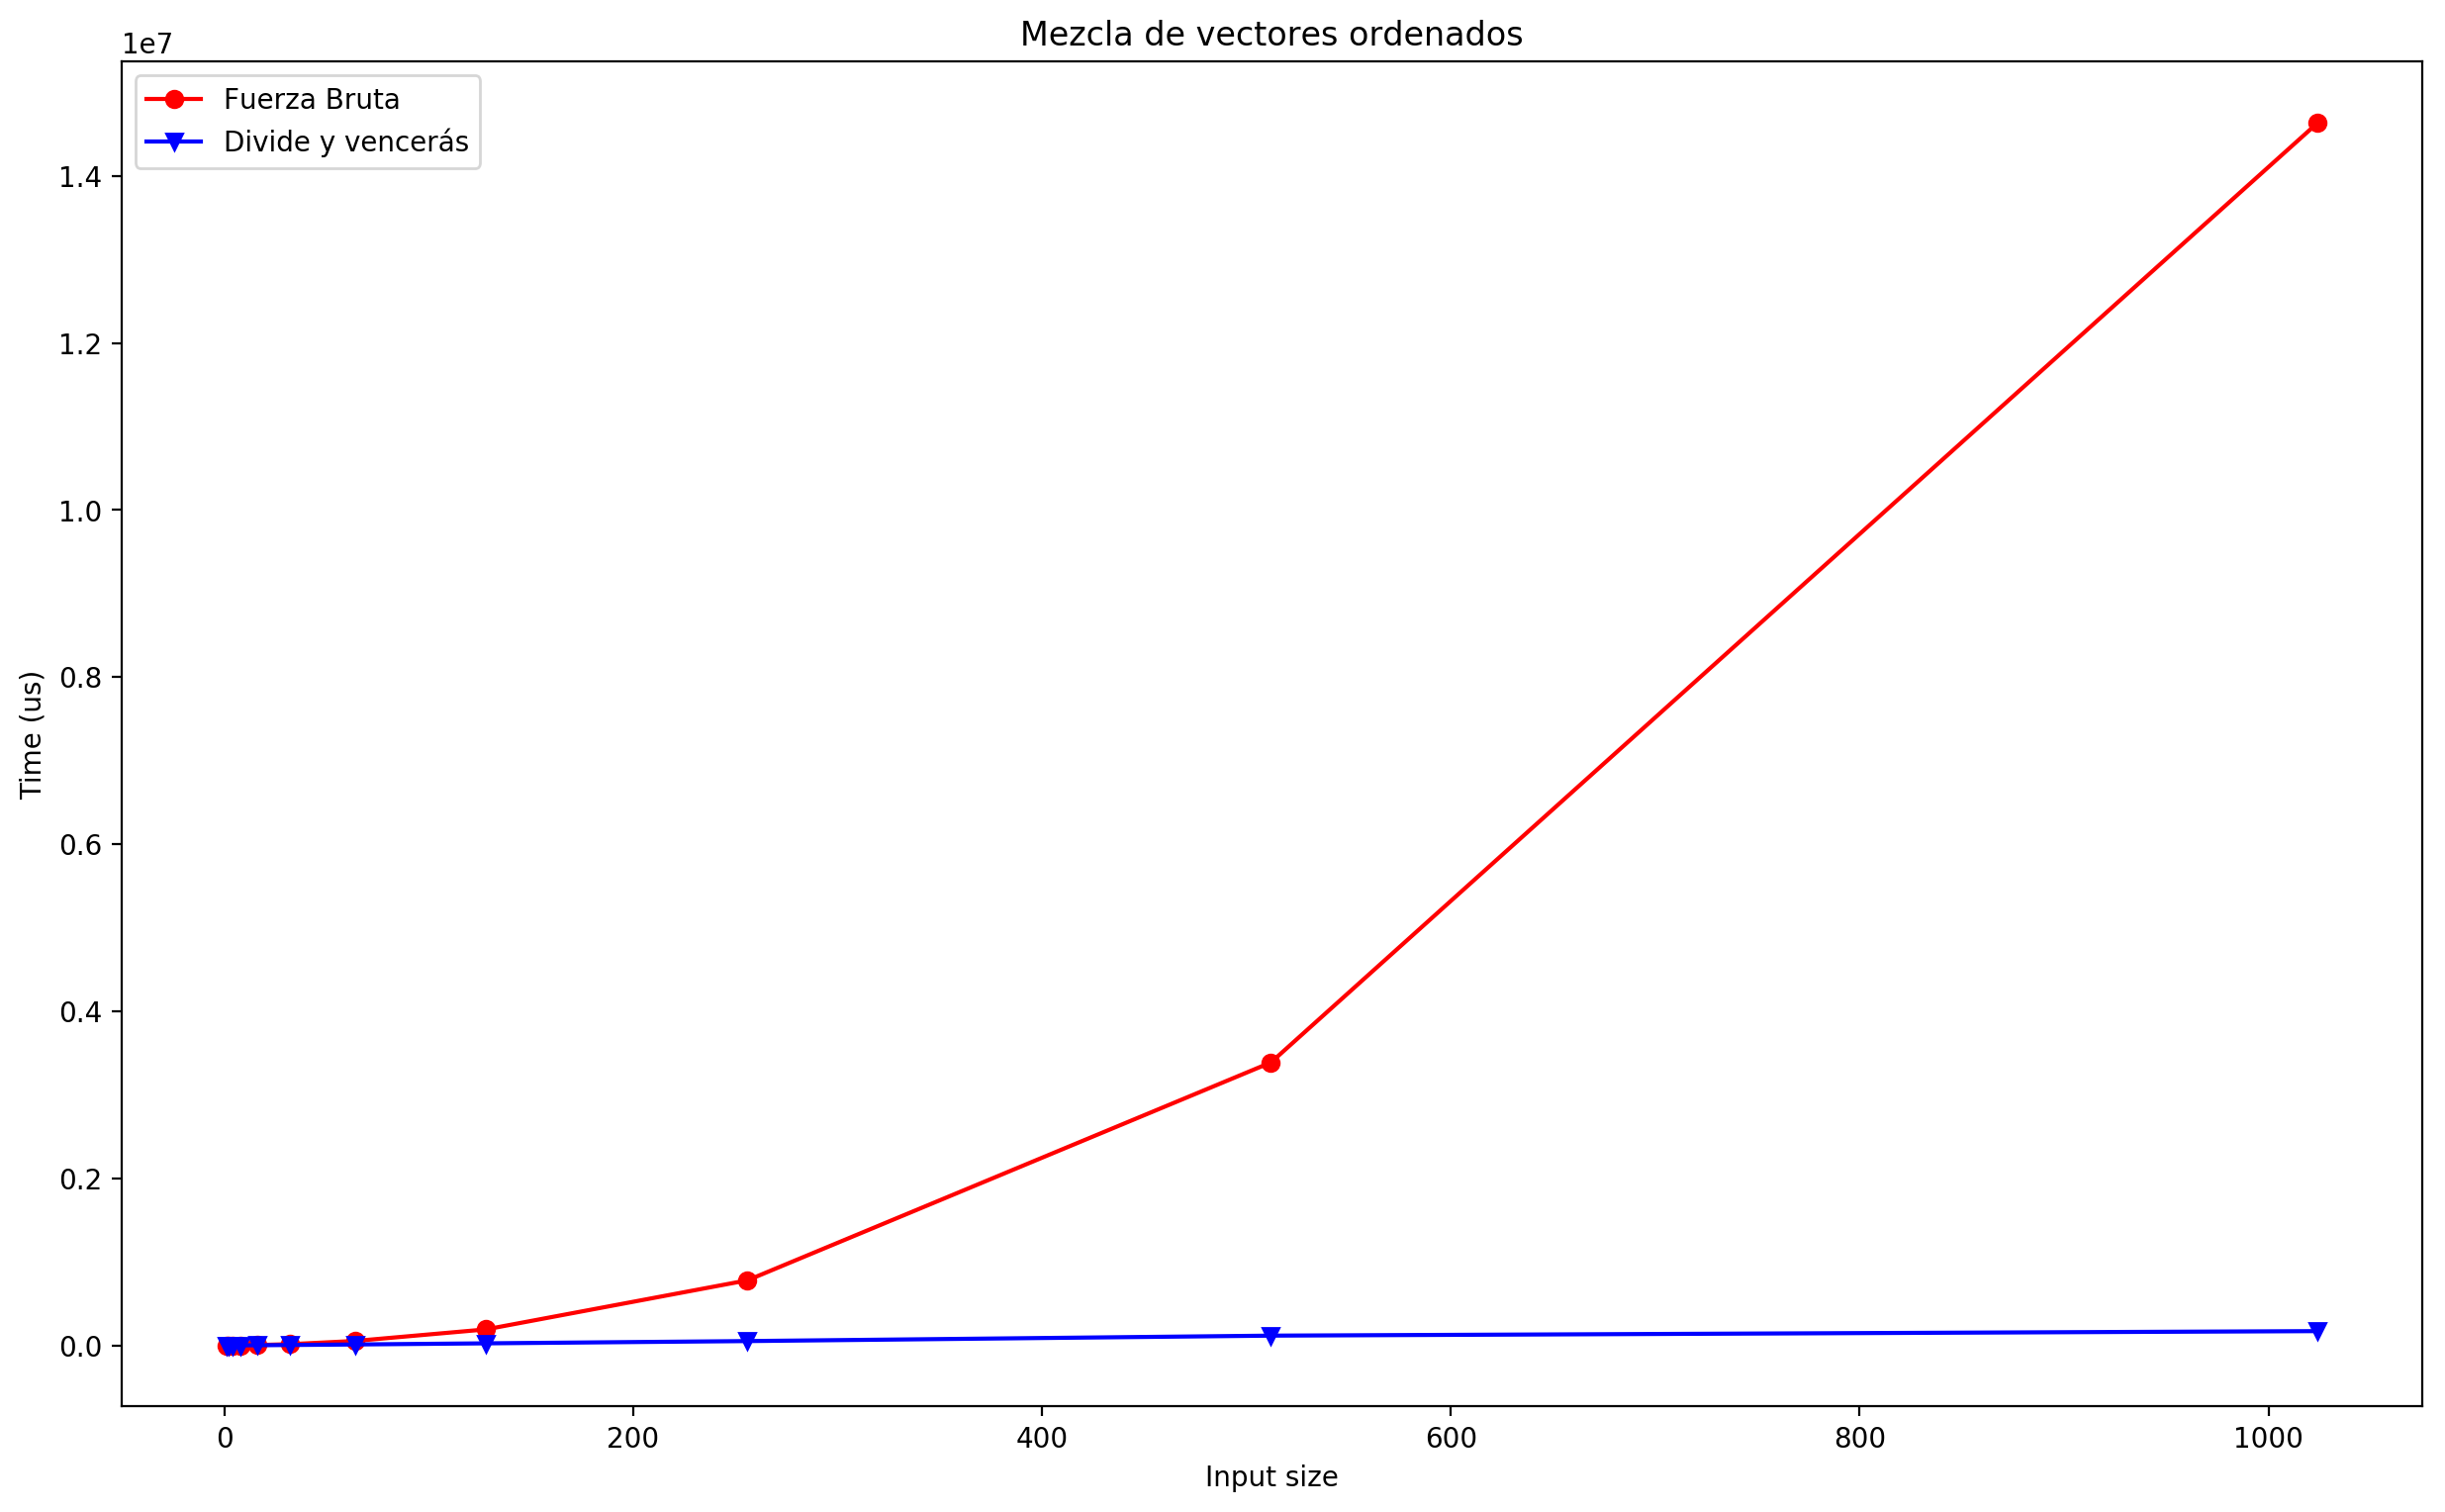
\includegraphics[width=\textwidth]{./Graficas/merge_ambos.png}
\end{frame}
\begin{frame}[fragile]{Mezclar \textit{k} vectores ordenados. \normalfont{Gráfica ambos zoom}}
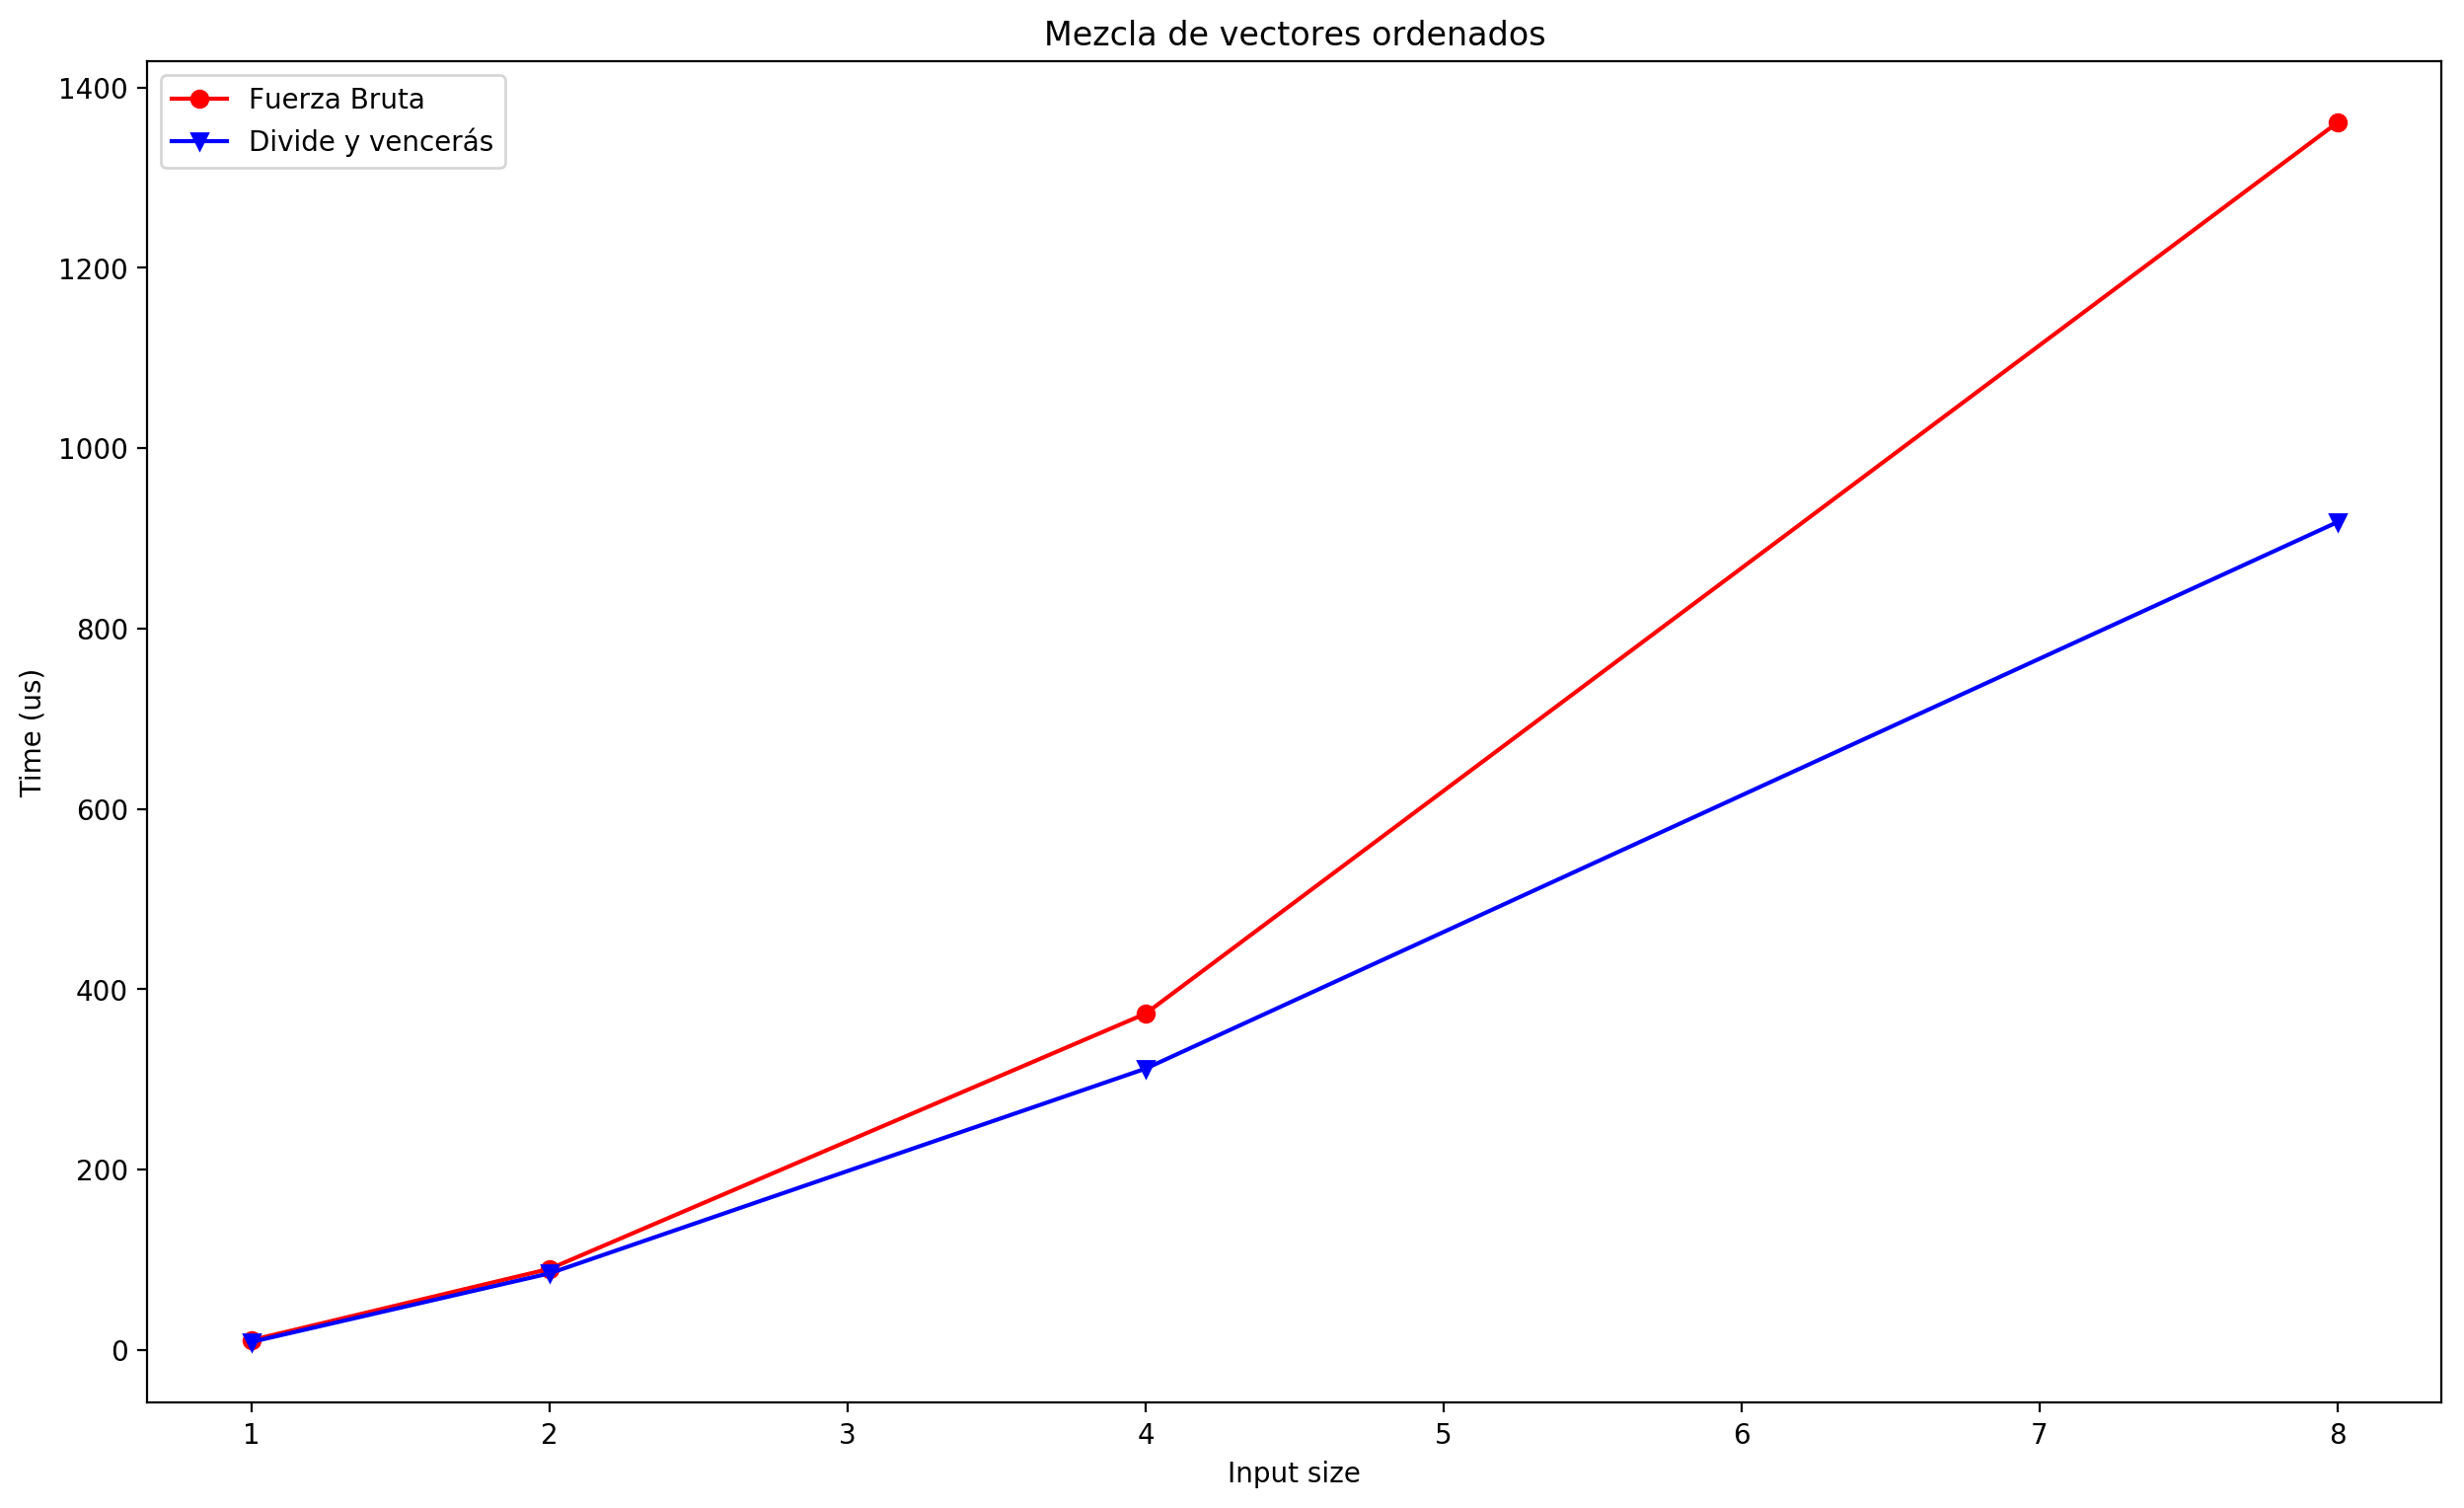
\includegraphics[width=\textwidth]{./Graficas/merge_ambos_zoom.png}
\end{frame}
\begin{frame}[fragile]{Mezclar \textit{k} vectores ordenados. \normalfont{Estudio del umbral}}
En la gráfica anterior podemos ver que el punto de corte de ambas gráficas es 2.
\newline
Por lo que podemos afirmar que el umbral es 2.

\newline Además hemos calculado dicho valor analíticamente.
\end{frame}


\section{Conclusión}

\begin{frame}{Conclusión}
Podemos observar que la técnica Divide y Vencerás no funciona en algunos casos, como es el de trasponer matrices. Sin embargo, nos ofrece un código con mejor legibilidad y con una consistencia mayor a la hora de mantenerlo.

Por ello es de máxima importancia el análisis, tanto empírico como teórico, previo a la utilización de dicho algoritmo.

\end{frame}



\end{document}
